\documentclass[12pt]{article}
\usepackage[paperwidth=48in,paperheight=36in,margin=0.55in]{geometry}
\usepackage[T1]{fontenc}
\usepackage[scaled=0.96]{helvet}
\renewcommand{\familydefault}{\sfdefault}
\usepackage{graphicx}
\usepackage{booktabs}
\usepackage{tabularx}
\usepackage{array}
\usepackage{enumitem}
\usepackage{colortbl}
\usepackage{xcolor}
\usepackage[hidelinks]{hyperref}
\usepackage{qrcode}
\usepackage{amsmath}
\usepackage{microtype}

\graphicspath{
  {figures/}
  {../outputs/alife_2026/editable_figures/}
  {../alife_lba_bundle/figures/}
  {../outputs/alife_2026/rule_diagrams/}
  {../figures/}
}

\pagestyle{empty}
\setlength{\parindent}{0pt}
\setlength{\parskip}{0.34em}
\setlist[itemize]{leftmargin=1.05em, itemsep=0.18em, topsep=0.18em}
\setlength{\tabcolsep}{8pt}
\renewcommand{\arraystretch}{1.20}

\definecolor{PosterBg}{HTML}{EFE2D0}
\definecolor{PosterPaper}{HTML}{FFFFFF}
\definecolor{PosterInk}{HTML}{3B3B3B}
\definecolor{PosterAccent}{HTML}{B00300}
\definecolor{PosterAccentSoft}{HTML}{FCDEB9}
\definecolor{PosterGray}{HTML}{5F5F5F}
\definecolor{PosterBorder}{HTML}{DBDBDB}
\definecolor{PosterMuted}{HTML}{E2E2E2}

\arrayrulecolor{PosterBorder}

\newcommand{\SectionHeader}[1]{%
  \vspace{0.32em}%
  \noindent\colorbox{PosterAccentSoft}{%
    \parbox{\dimexpr\linewidth-2\fboxsep\relax}{%
      \vspace{0.18em}\color{PosterAccent}\fontsize{26}{30}\selectfont\bfseries #1\vspace{0.16em}%
    }%
  }%
  \vspace{0.28em}%
}

\newcommand{\LeadBox}[1]{%
  \noindent\fcolorbox{PosterBorder}{PosterAccentSoft}{%
    \parbox{\dimexpr\linewidth-2\fboxsep-2\fboxrule\relax}{%
      \vspace{0.22em}\fontsize{20}{24}\selectfont #1\vspace{0.20em}%
    }%
  }%
}

\newcommand{\PosterCard}[1]{%
  \noindent\fcolorbox{PosterBorder}{PosterPaper}{%
    \parbox{\dimexpr\linewidth-2\fboxsep-2\fboxrule\relax}{#1}%
  }%
}

\begin{document}
\pagecolor{PosterBg}
\color{PosterInk}
\fontsize{21}{27}\selectfont

\noindent
\colorbox{PosterAccent}{%
  \parbox{\dimexpr\textwidth-2\fboxsep\relax}{%
    \vspace{0.24in}
    {\color{white}\fontsize{68}{72}\selectfont\bfseries Bernoulli NML Selects Relative-Periodic Domains\par}
    \vspace{0.08in}
    {\color{PosterAccentSoft}\fontsize{30}{34}\selectfont Residual defect masks expose persistent structure in cellular automaton spacetime\par}
    \vspace{0.10in}
    {\color{white}\fontsize{22}{26}\selectfont Joshua Herman\hfill ALIFE 2026\hfill Affiliation to be added\par}
    \vspace{0.20in}
  }%
}

\vspace{0.30em}
\LeadBox{\textbf{Main result.} A single complexity-penalized selector fits a global periodic scaffold in 1D, 2D, and 3D cellular automata. The strongest 2D cases do not collapse to noise after background subtraction; they leave low-density residual masks that stay visibly structured.}

\vspace{0.45em}
\noindent
\begin{minipage}[t]{0.285\textwidth}

\SectionHeader{Problem}
Broad CA domains coexist with particles, interfaces, and other persistent defects. The practical task is to choose \emph{which global period and shift best explain a finite observed spacetime}.

\LeadBox{\textbf{Poster lens.} Fit the scaffold first, then study what survives in the residual.}

\SectionHeader{Selector}
\begin{itemize}
  \item Translation by $(t,\mathbf{x}) \mapsto (t+p,\mathbf{x}+\mathbf{s})$ induces orbit classes.
  \item Majority vote on each orbit gives the nearest background $B^*(p,\mathbf{s})$.
  \item The residual mask is $M = U \oplus B^*(p,\mathbf{s})$.
  \item Bernoulli NML compares candidate periods and shifts without rewarding unnecessary template size.
\end{itemize}

\[
\mathrm{NML}(p,\mathbf{s}) =
\sum_j n_j H_b(\hat{\theta}_j)
\;+\;
\frac{1}{2}\sum_j \log_2 n_j
\]

The fit term favors pure orbit classes. The penalty prevents larger templates from winning by sheer flexibility.

\vspace{0.18em}
\PosterCard{
  \vspace{0.10em}
  
\includegraphics[width=\linewidth]{algorithm_detailed_tikz.pdf}
  \vspace{0.06em}
}

\SectionHeader{Why Not Raw Likelihood?}
\PosterCard{
  {\fontsize{18}{22}\selectfont
  \begin{tabularx}{\linewidth}{@{}lX@{}}
  \toprule
  Selector & Outcome on 105 nontrivial LifeWiki rules at $T=100$ \\
  \midrule
  Residual minimization & 16 pick $p=1$, 8 pick $p=2$, and 81 pick period $\ge 4$ \\
  Bernoulli NLL & All 105 pick the maximum tested period \\
  Bernoulli NML & 97 pick $p=1$, 7 pick $p=2$, and 1 picks $p=8$ \\
  \bottomrule
  \end{tabularx}
  }
}

\vspace{0.18em}
Bernoulli NML is the useful poster-side argument: without the complexity term, the selector overfits almost immediately.

\end{minipage}\hfill
\begin{minipage}[t]{0.415\textwidth}

\SectionHeader{2D Main Result}
Observed, background, and defect panels separate what the scaffold explains from what remains structured after subtraction.

\PosterCard{
  \vspace{0.12em}
  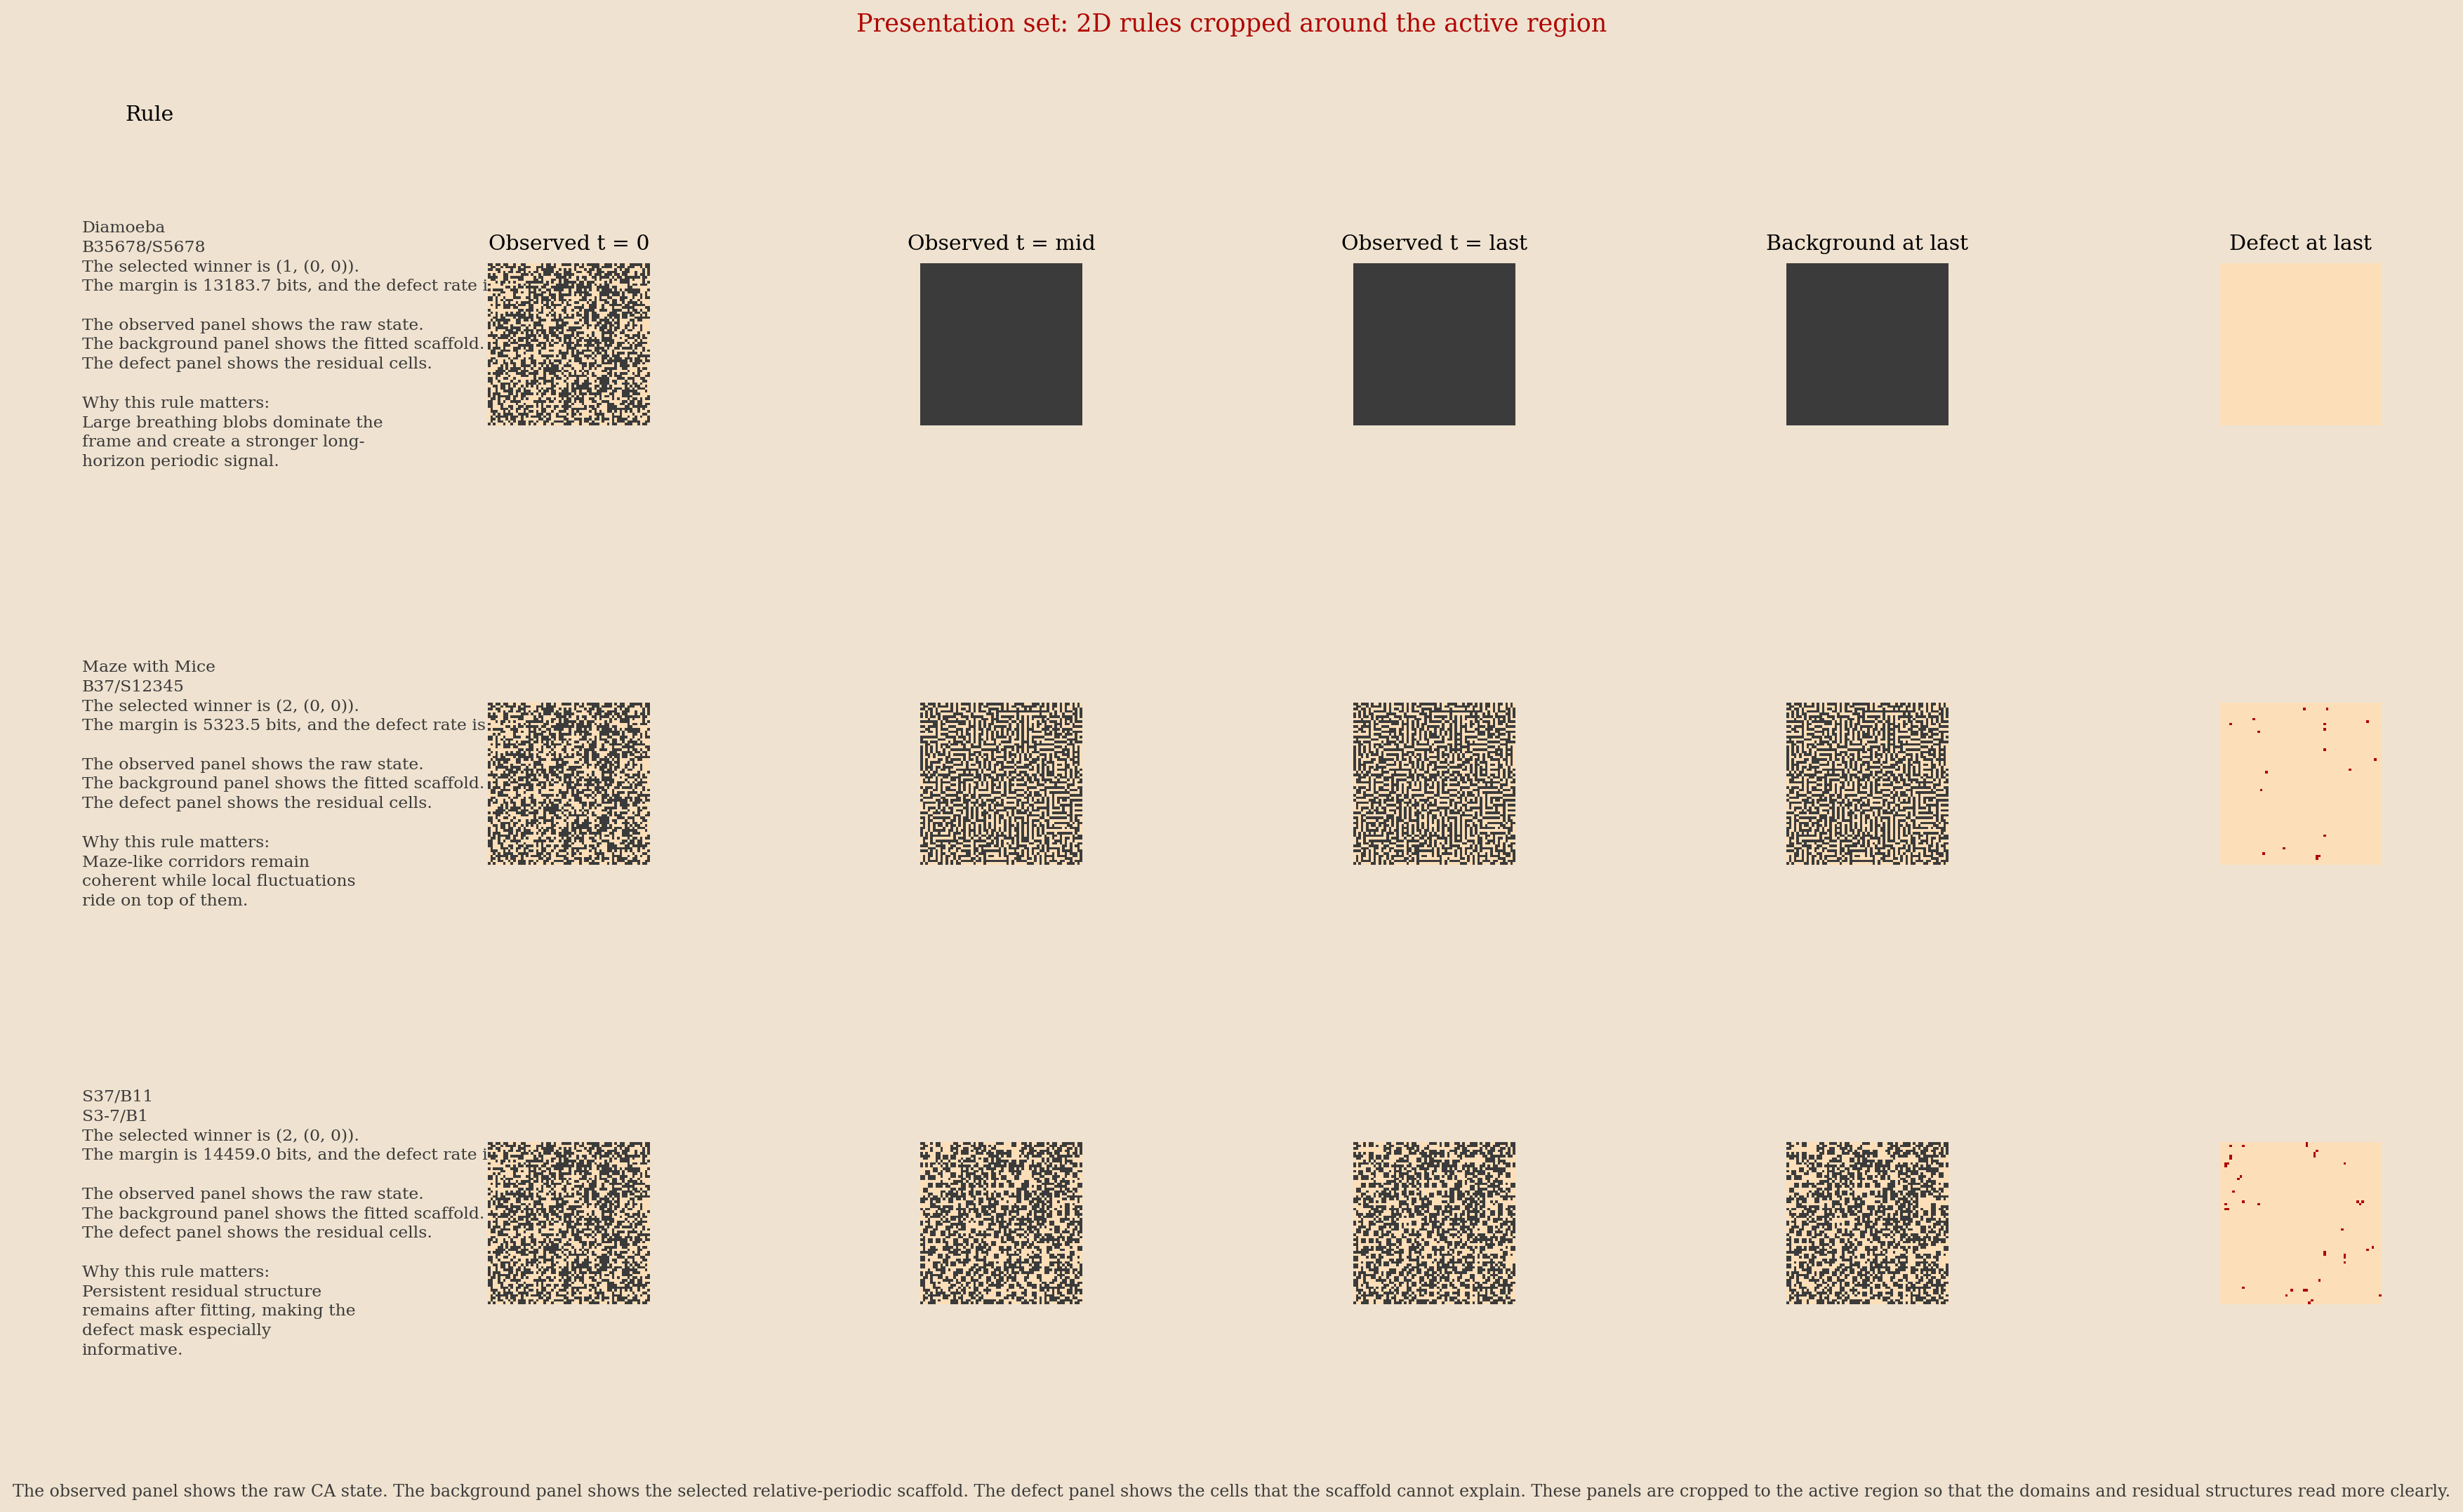
\includegraphics[width=\linewidth]{presentation_rules_2d.png}
  \vspace{0.05em}
}

\vspace{0.24em}
\LeadBox{\textbf{Most important visual claim.} In 2D, the selected scaffold captures broad regular domains while residual masks preserve coherent, low-density structure. The method is therefore useful both for selection and for downstream defect analysis.}

\SectionHeader{Focal 2D Cases}
\begin{itemize}
  \item \textbf{Diamoeba}: large breathing domains, selected winner $(p,\mathbf{s})=(1,(0,0))$, defect rate $0.077$.
  \item \textbf{Maze with Mice}: highly coherent maze background, selected winner $(2,(0,0))$, defect rate $0.008$.
  \item \textbf{S37/B11}: low-defect background plus persistent residual structure, selected winner $(2,(0,0))$, defect rate $0.015$ in the presentation run.
\end{itemize}

\SectionHeader{Cross-Dimensional Checks}
\PosterCard{
  \begin{minipage}[t]{0.49\linewidth}
  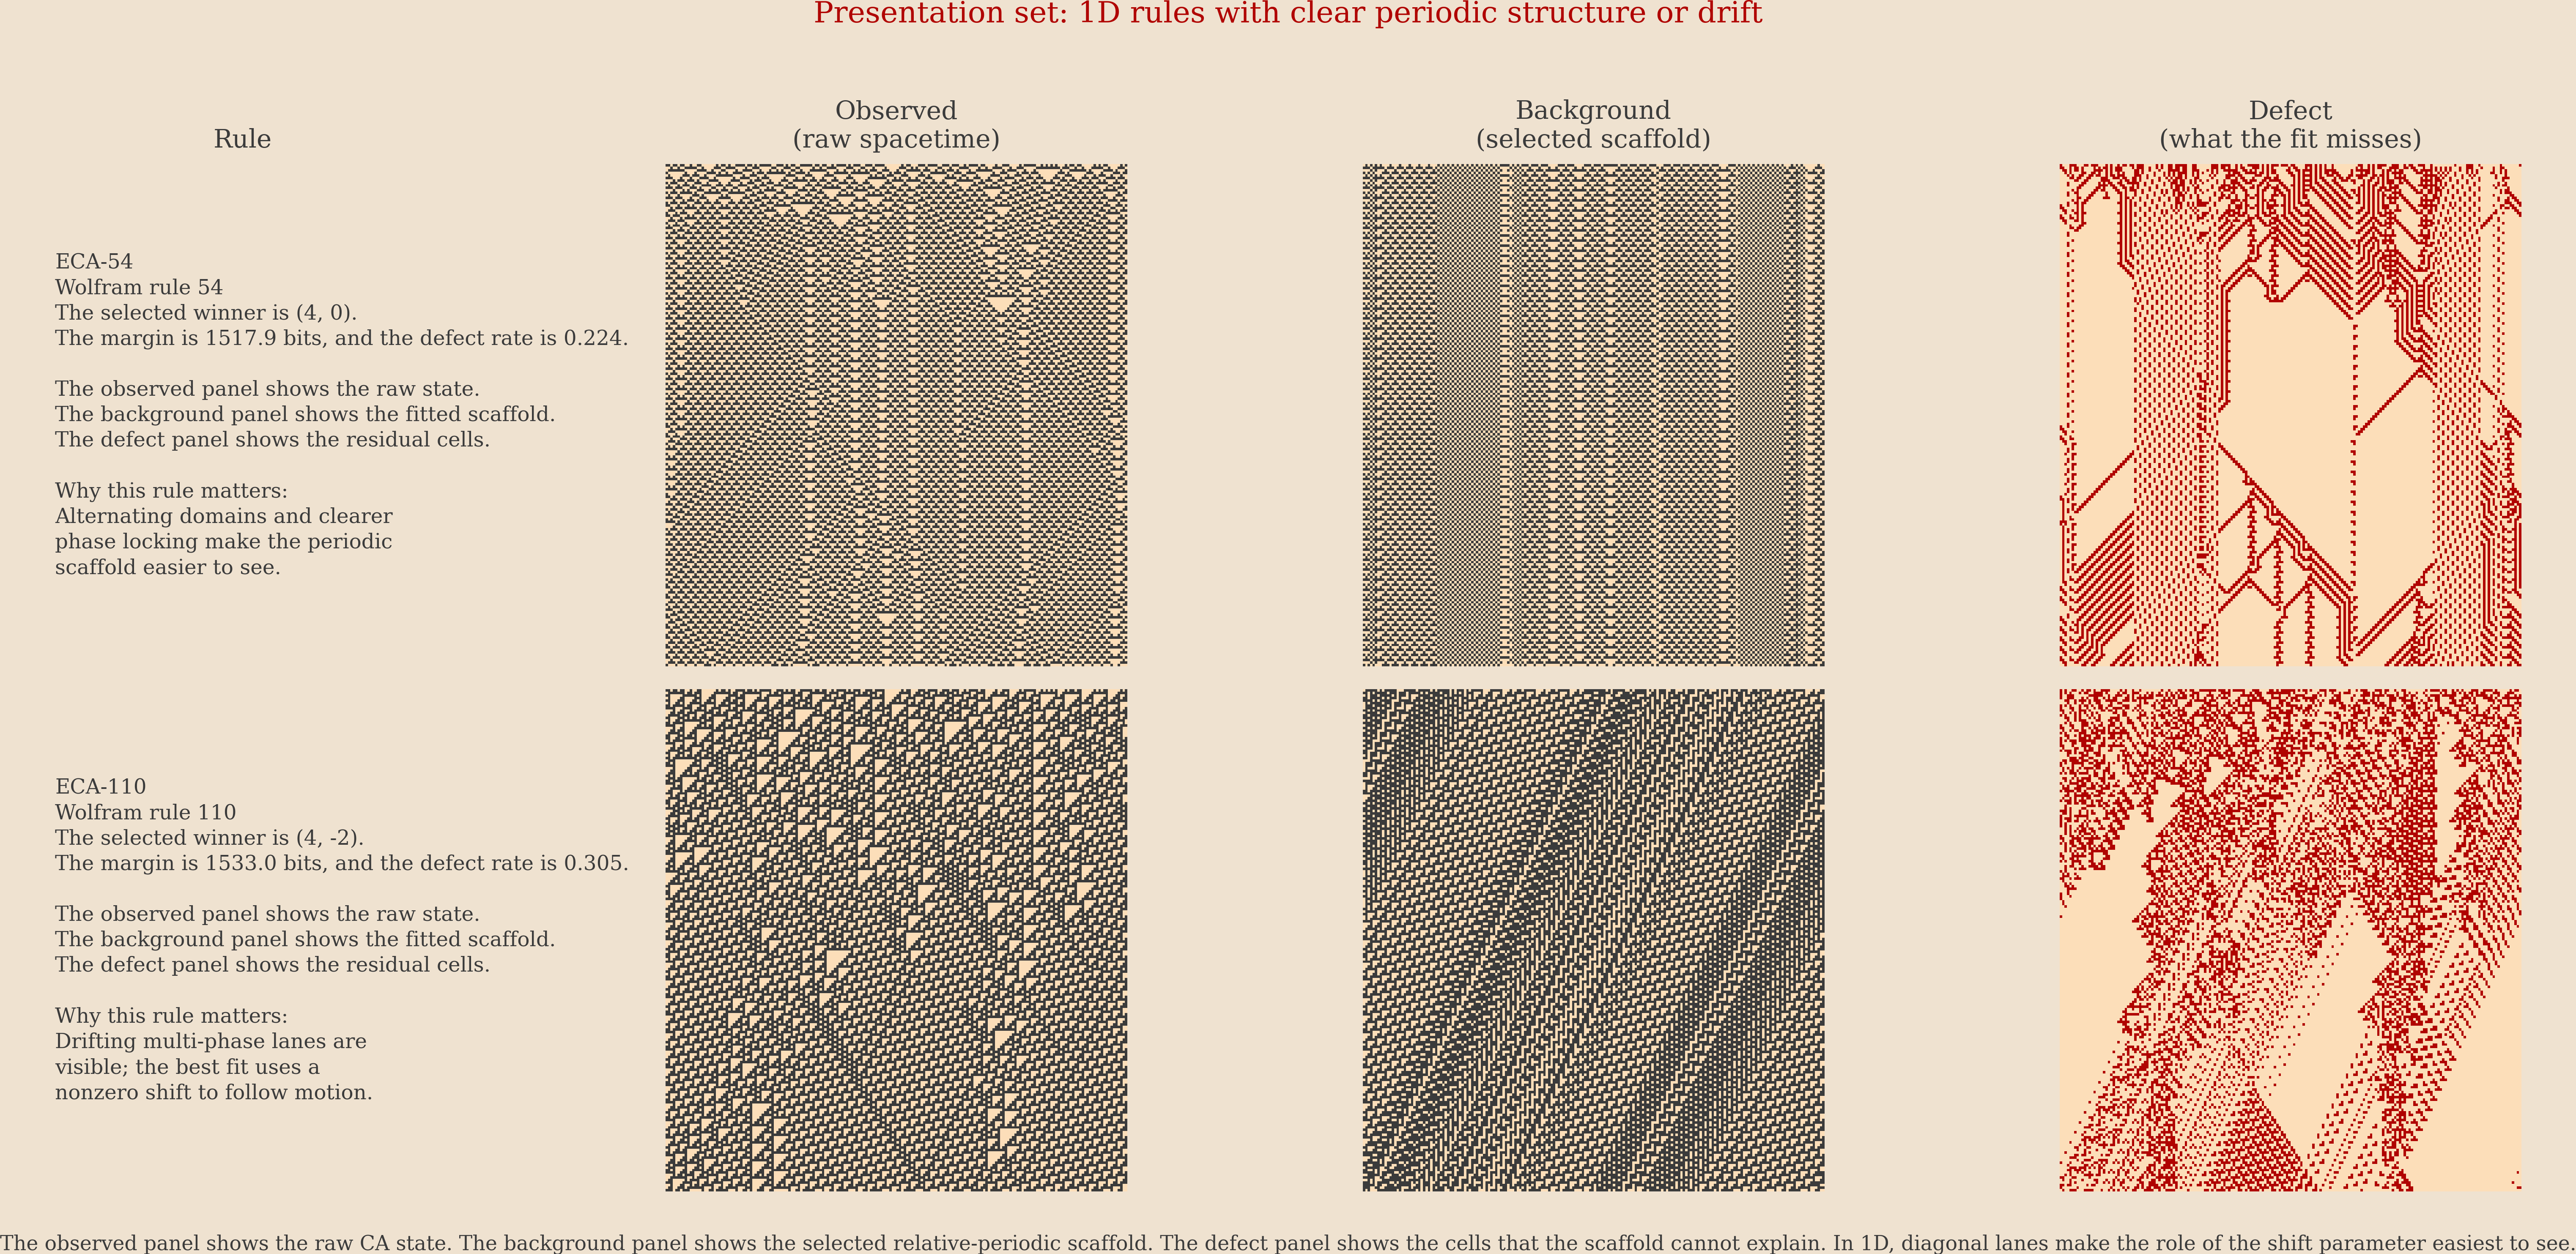
\includegraphics[width=\linewidth]{presentation_rules_1d.png}
  \vspace{0.15em}

  {\fontsize{17}{21}\selectfont \textbf{1D.} ECA-54 locks to period $4$. ECA-110 stabilizes to $(p,s)=(4,-2)$ under the period-first selector.}
  \end{minipage}\hfill
  \begin{minipage}[t]{0.49\linewidth}
  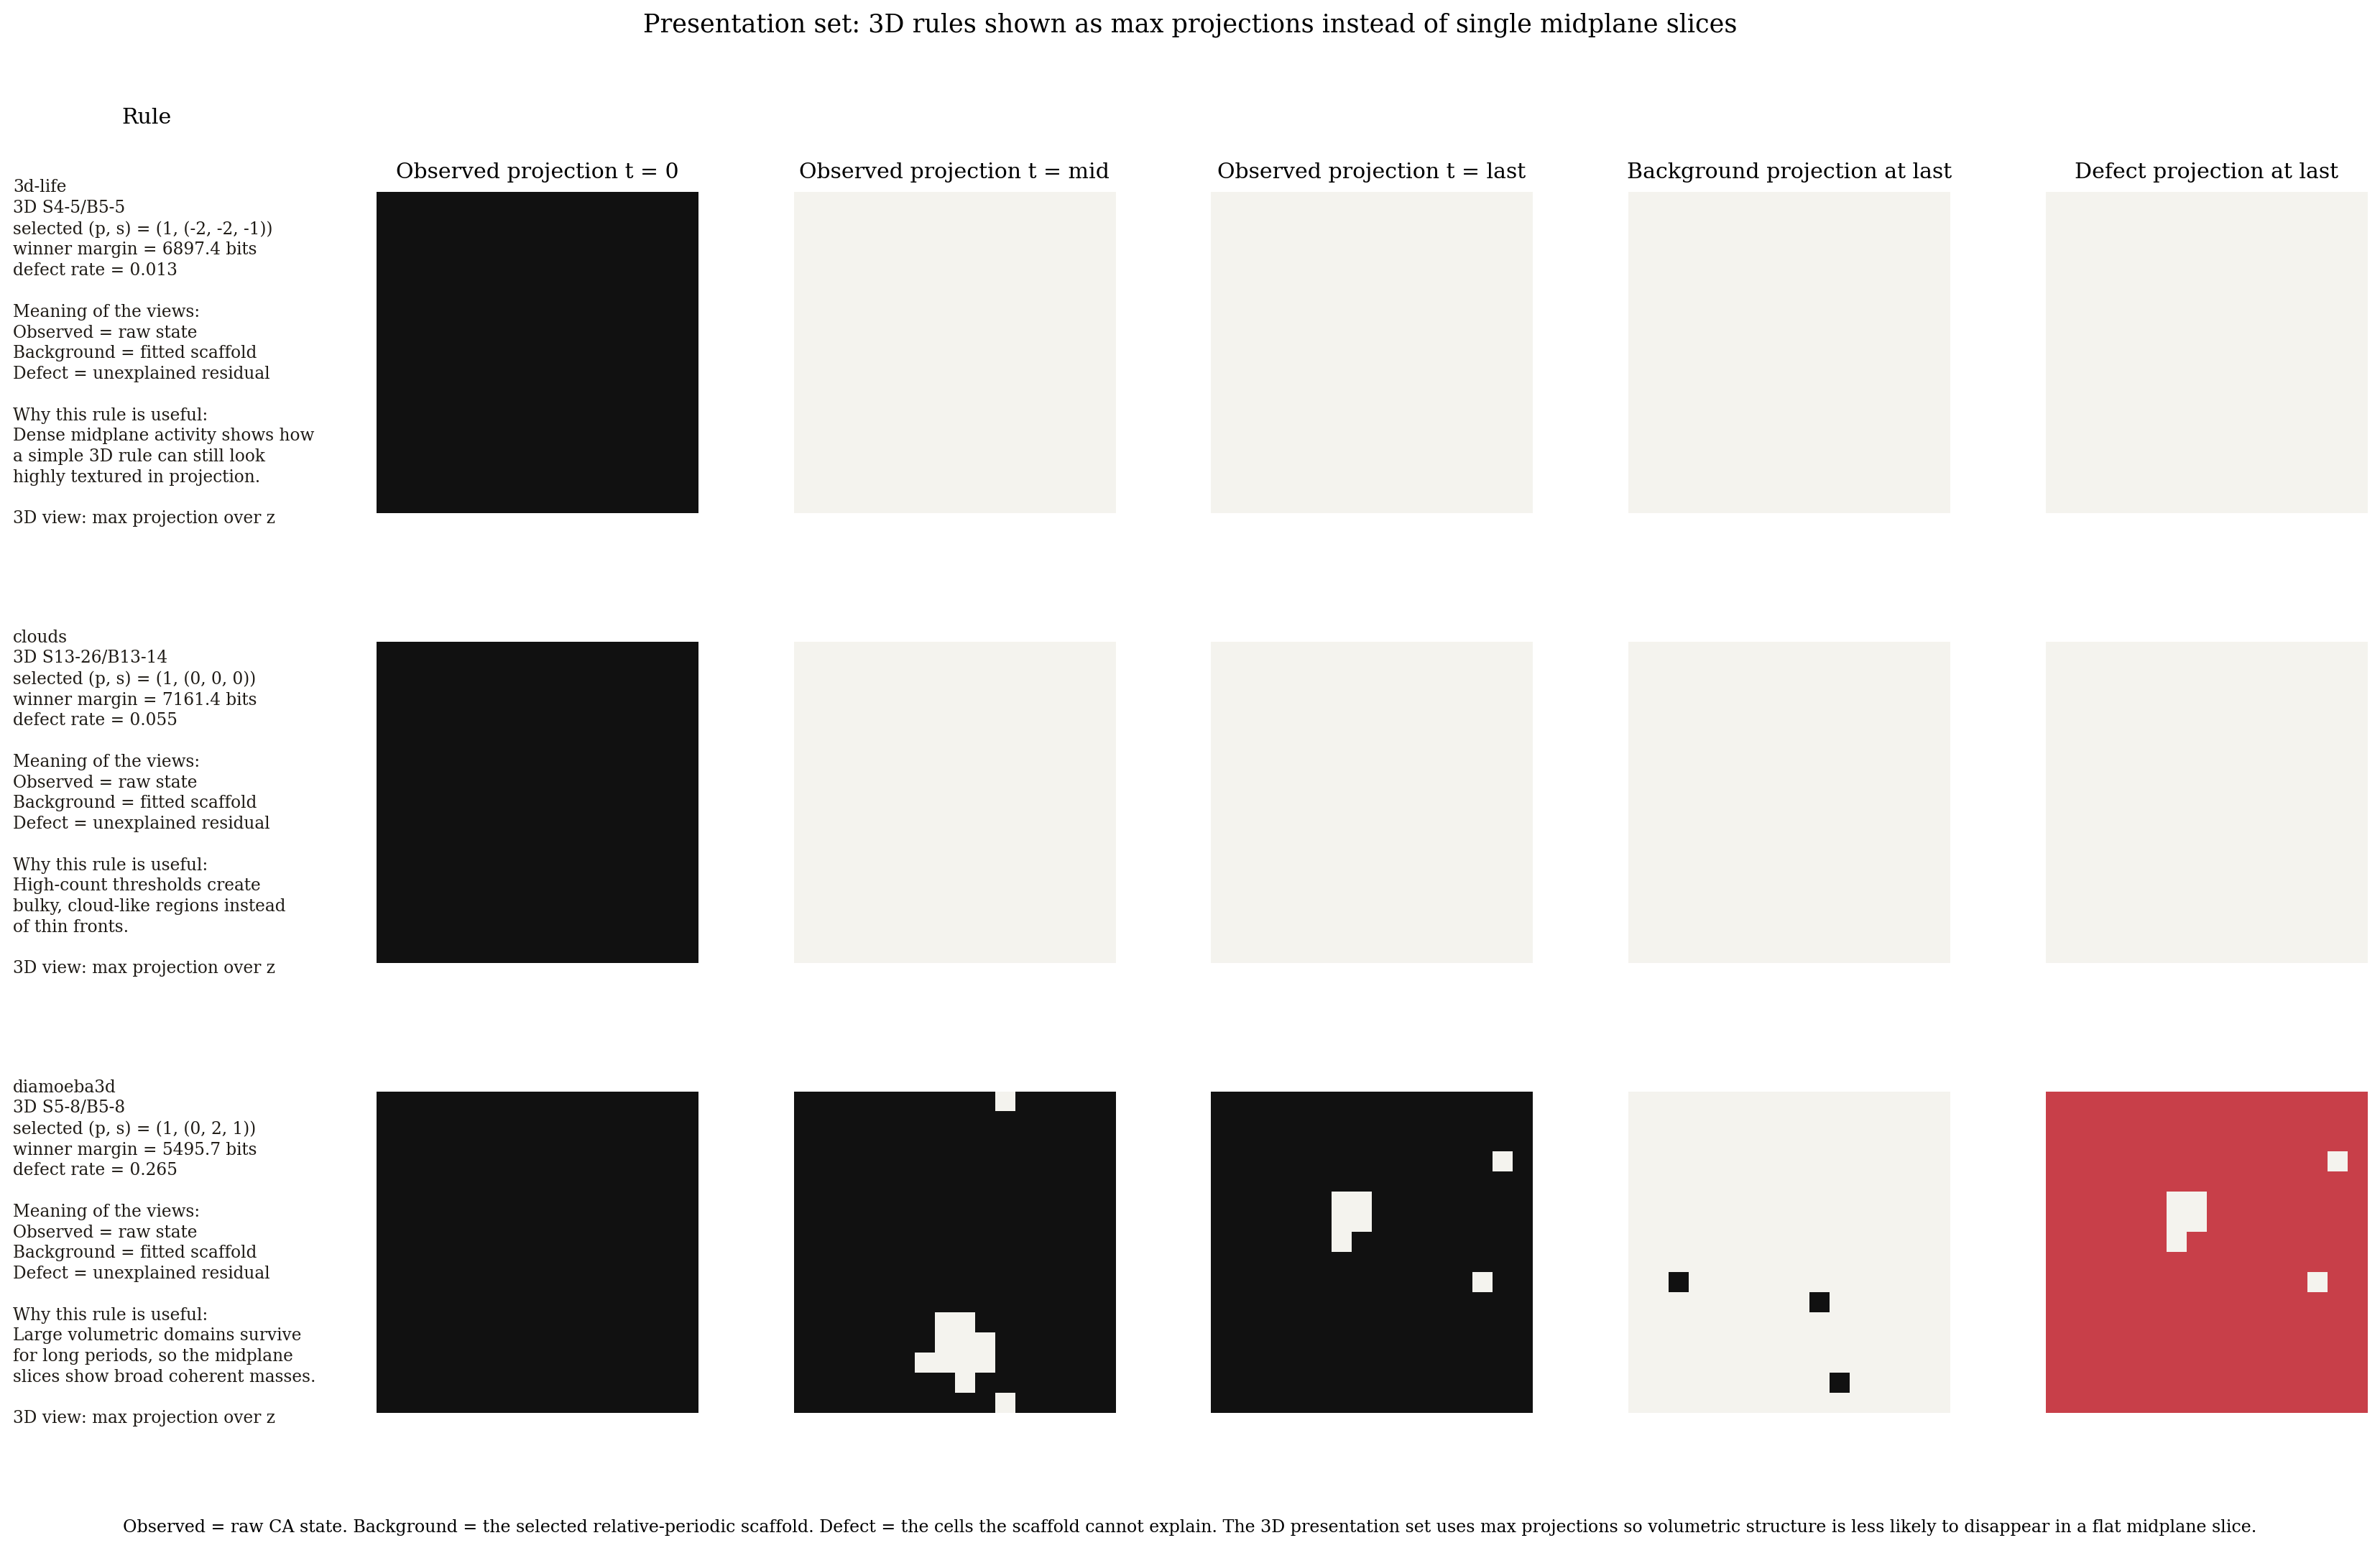
\includegraphics[width=\linewidth]{presentation_rules_3d.png}
  \vspace{0.15em}

  {\fontsize{17}{21}\selectfont \textbf{3D.} The same decomposition still works on volumetric rules; the tested diamoeba3d case settles to period $1$.}
  \end{minipage}
}

\end{minipage}\hfill
\begin{minipage}[t]{0.285\textwidth}

\SectionHeader{Stability Across Horizon}
The selected period usually locks quickly as the observation horizon grows.

\PosterCard{
  \vspace{0.10em}
  
\includegraphics[width=\linewidth]{stabilization_summary.pdf}
  \vspace{0.04em}
}

\begin{itemize}
  \item \textbf{ECA-54} locks immediately to period $4$.
  \item \textbf{ECA-110} passes through a short transient and then locks to period $4$ with shift $-2$.
  \item \textbf{S24/B11} changes later, as longer horizons reveal additional periodic structure.
  \item \textbf{Diamoeba3d} corrects a small-sample transient and then locks to period $1$.
\end{itemize}

\SectionHeader{Controls And Robustness}
\PosterCard{
  {\fontsize{18}{22}\selectfont
  \begin{tabularx}{\linewidth}{@{}l>{\raggedleft\arraybackslash}p{1.10in}>{\raggedleft\arraybackslash}p{1.10in}@{}}
  \toprule
  2D summary & Mean period & Mean defect rate \\
  \midrule
  Original runs & 2.2 & 0.014 \\
  Bernoulli i.i.d. & 1.0 & 0.384 \\
  Space shuffled & 1.0 & 0.384 \\
  Time shuffled & 1.0 & 0.114 \\
  \bottomrule
  \end{tabularx}
  }
}

\vspace{0.16em}
Shuffled and i.i.d. controls collapse back toward period $1$ and much worse defect rates, which is consistent with the selector responding to real spacetime structure rather than generic occupancy statistics.

\vspace{0.18em}
\PosterCard{
  {\fontsize{18}{22}\selectfont
  \begin{tabularx}{\linewidth}{@{}l>{\raggedleft\arraybackslash}p{0.85in}>{\raggedleft\arraybackslash}p{0.95in}>{\raggedleft\arraybackslash}X@{}}
  \toprule
  Rule & Modal $p$ & Defect rate & Seed consistency \\
  \midrule
  S14/B11 & 1 & 0.0059 & 10 / 10 \\
  S24/B11 & 2 & 0.0278 & 10 / 10 \\
  S37/B11 & 2 & 0.0441 & 10 / 10 \\
  S11/B37 & 4 & 0.0275 & 7 / 10 \\
  \bottomrule
  \end{tabularx}
  }
}

\vspace{0.16em}
For \textbf{S37/B11}, the late defect density stays close to $0.011$ across $32^2$ to $192^2$ grids, with mean late defects growing from $11.4$ to $428.5$.

\SectionHeader{Takeaways}
\LeadBox{
\begin{itemize}
  \item A single global selector gives usable periodic scaffolds in 1D, 2D, and 3D CA.
  \item The complexity penalty changes the selected period qualitatively; it is not cosmetic.
  \item In 2D, residual masks expose structured defects and make broad surveys feasible.
  \item The method is a front end for richer local analysis, not a replacement for computational mechanics.
\end{itemize}
}

\end{minipage}

\vspace{0.45em}
\noindent\fcolorbox{PosterBorder}{PosterPaper}{%
  \parbox{\dimexpr\textwidth-2\fboxsep-2\fboxrule\relax}{%
    \begin{minipage}[t]{0.78\textwidth}
    {\fontsize{15}{19}\selectfont
    \textbf{Design notes for this version.} The poster uses the ALIFE 2026 site palette: accent-1 beige background, accent-2 deep red, pale apricot highlight, and charcoal neutrals. Text was enlarged and sections were simplified to support fast scanning at distance.

    \vspace{0.20em}
    \textbf{Selected sources inside this repo.} Algorithm figure: \texttt{poster/figures/algorithm\_detailed\_tikz.tex}. Stabilization figure: \texttt{scripts/alife\_stabilization\_summary.py}. Presentation panels: \texttt{outputs/alife\_2026/rule\_diagrams}. Control summaries: \texttt{outputs/alife\_2026/null\_controls}. Multi-seed and scaling summaries: \texttt{outputs/strengthening\_v2}.

    \vspace{0.20em}
    \textbf{Project link.} \url{https://github.com/zitterbewegung/relative_symmetry_repair}
    }
    \end{minipage}\hfill
    \begin{minipage}[t]{0.18\textwidth}
    \raggedleft
    \qrcode[height=1.45in]{https://github.com/zitterbewegung/relative_symmetry_repair}

    {\fontsize{13}{16}\selectfont
    Scan for repo, paper assets, and scripts.\\
    Replace with a preprint URL if needed.
    }
    \end{minipage}
  }%
}

\end{document}
